\documentclass[english]{tktltiki}
\usepackage[pdftex]{graphicx}
\usepackage{subfigure}
\usepackage{url}
\begin{document}
%\doublespacing
%\singlespacing
\onehalfspacing

\title{Assignment 1: Improvement of the interaction of a website}
\author{P�ter Ivanics}
\date{\today}

\maketitle

\numberofpagesinformation{\numberofpages\ pages + \numberofappendixpages\ appendices}
\keywords{}

\mytableofcontents

\section{Introduction}
	This short report contains a heuristic evaluation and improvement of a simple one-page website. The report is rolled out as one of the assignment of the Human-Computer Interaction course and serves the purpose to gain hands-on experience with the course material. The given webpage of discussion is displayed on Figure \ref{original_webpage}. 
	
	\begin{figure}[h] 
		\begin{center}
			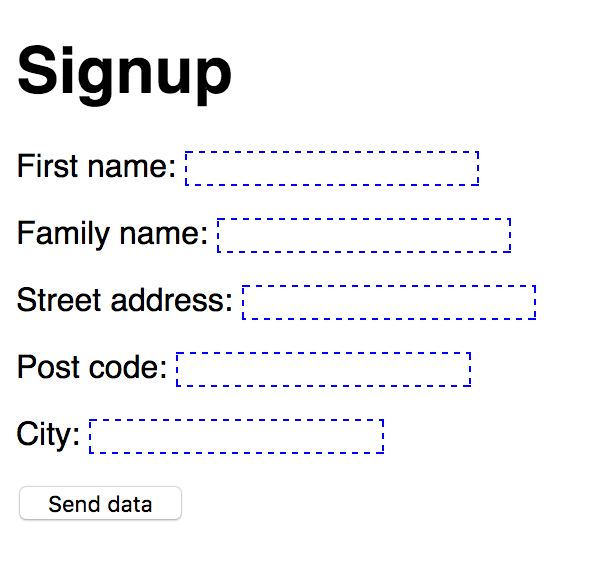
\includegraphics[height=0.6\textwidth]{images/original_webpage.png}
			\caption{The webpage of discussion in its original state, that is going to be analyzed and improved in this report.}
			\label{original_webpage}
		\end{center}
	\end{figure}

	As shown, the webpage includes a very simple web form with the purpose of user registration for a service .The page has a title of "Online shop -- Registration", a couple of labels and textboxes and a button in the bottom which is supposed to validate and submit the data if all fields are filled correctly by the user. The next chapter of this report describes the heuristic evaluation of the website, which means listing the proposed suggestions, improvement possibilities, design ideas and features for this simple form. Further, a short description about the implementation is given which is based on the former evaluation. Finally, the last chapter concludes the report and describes further improvement possibilities for the website. 

\section{Heuristic evaluation}

% [description of the usability characteristics used, and UI improvements planned based on them]
	To set the context, the term of heuristic evaluation is defined shortly. As discussed on the lecture, heuristic evaluation is one of the possible methods for performing usability testing of a website or system. The heuristic method means performing the evaluation without end-user involvement. This is done on the given single page with the utilization of the discussed usability characteristics and explanation on User Centered Design (UCD) during the lecture.
	
	 To begin the analysis with, the original form displayed on Figure \ref{original_webpage} is as minimalistic as possible. In general this should not be considered as a problem, but rather as a possibility, because this observation gives a lot of room for improvements. Taking the first look at the original webpage, one can immediately see what it is about - the user is expected to provide certain information about him/herself to sign up for a service. Nevertheless, one notices soon that this page does not correspond to today's standards, the page is not optimized for mobile devices and usability can be greatly enhanced by applying some simple modifications. Due to the simplicity of the page, too many use-case scenarios cannot be investigated and therefore only the inspection of this screen is explained. The suggestions to follow are explained in importance order (from the most important to the least important). 
	 
	 The most important principle to point out during the improvement of a web page is the "Don't make me think" principle \cite{SK14}. To summarize in one sentence, the meaning is to keep the webpage as self-evident and obvious as possible. When a user is presented this page, they should immediately understand that 
	 
	\begin{enumerate}
		\item they are on a registration form, 
		\item what are they signing up for,
		\item what information are they required to give,
		\item what subset of the information is mandatory (i.e. which are the mandatory fields and which ones can be skipped),
		\item how do they submit that information,
		\item what happens after the information is submitted.
	\end{enumerate}
	
	

\section{Implementation}

% [description that helps the lecturer(s) to understand your solution; does not need to be long]

\section{Unimplemented features}

% [describe here the solutions that your web site does not have but which would be useful and important]

\nocite{*}
\bibliographystyle{tktl}
\bibliography{bibliography}

\lastpage

\appendices

\pagestyle{empty}

%\internalappendix{1}{Model ABC}
%
%The appendices here are just models of the table of contents and the presentation. Each appendix 
%usually starts on its own page, with the name and number of the appendix at the top. Each appendix is paginated separately.
%
%In addition to complementing the main document, each appendix is also its own, independent entity. 
%This means that an appendix cannot be just an image or a piece of programming, but the appendix must explain its contents and meaning.

\end{document}


